\section{Introducción}

\begin{frame}[t]{La ley de Moore}
\begin{columns}
  \begin{column}{.5\textwidth}
    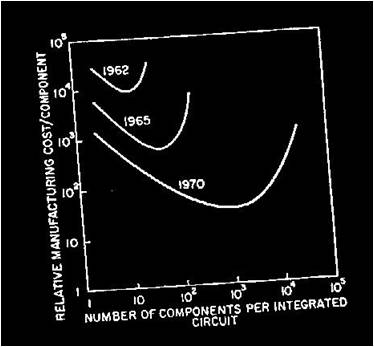
\includegraphics[width=.5\textwidth]{images/moore-graph1.jpg}\\
    \begin{flushright}
      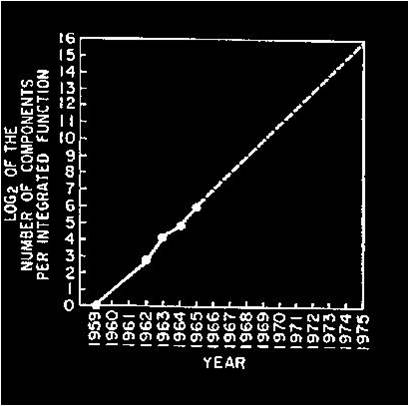
\includegraphics[width=.65\textwidth]{images/moore-graph2.jpg}\\
    \end{flushright}
  \end{column}
  \begin{column}{.5\textwidth}
    \begin{itemize}
    \item El número de transistores por chip se duplica cada N meses.
      \begin{itemize}
        \item Donde 12 \textless N \textless 24.
        \item Gordon Moore, 1965.
      \end{itemize}
    \end{itemize}
    \vspace{1em}
    \begin{center}
      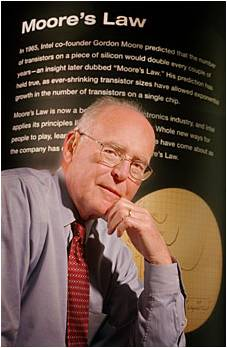
\includegraphics[width=.4\textwidth]{images/gordon-moore.jpg}
    \end{center}
  \end{column}
\end{columns}
\end{frame}



\begin{frame}[t]{Transistores por chip}
    \begin{center}
      \mode<presentation>{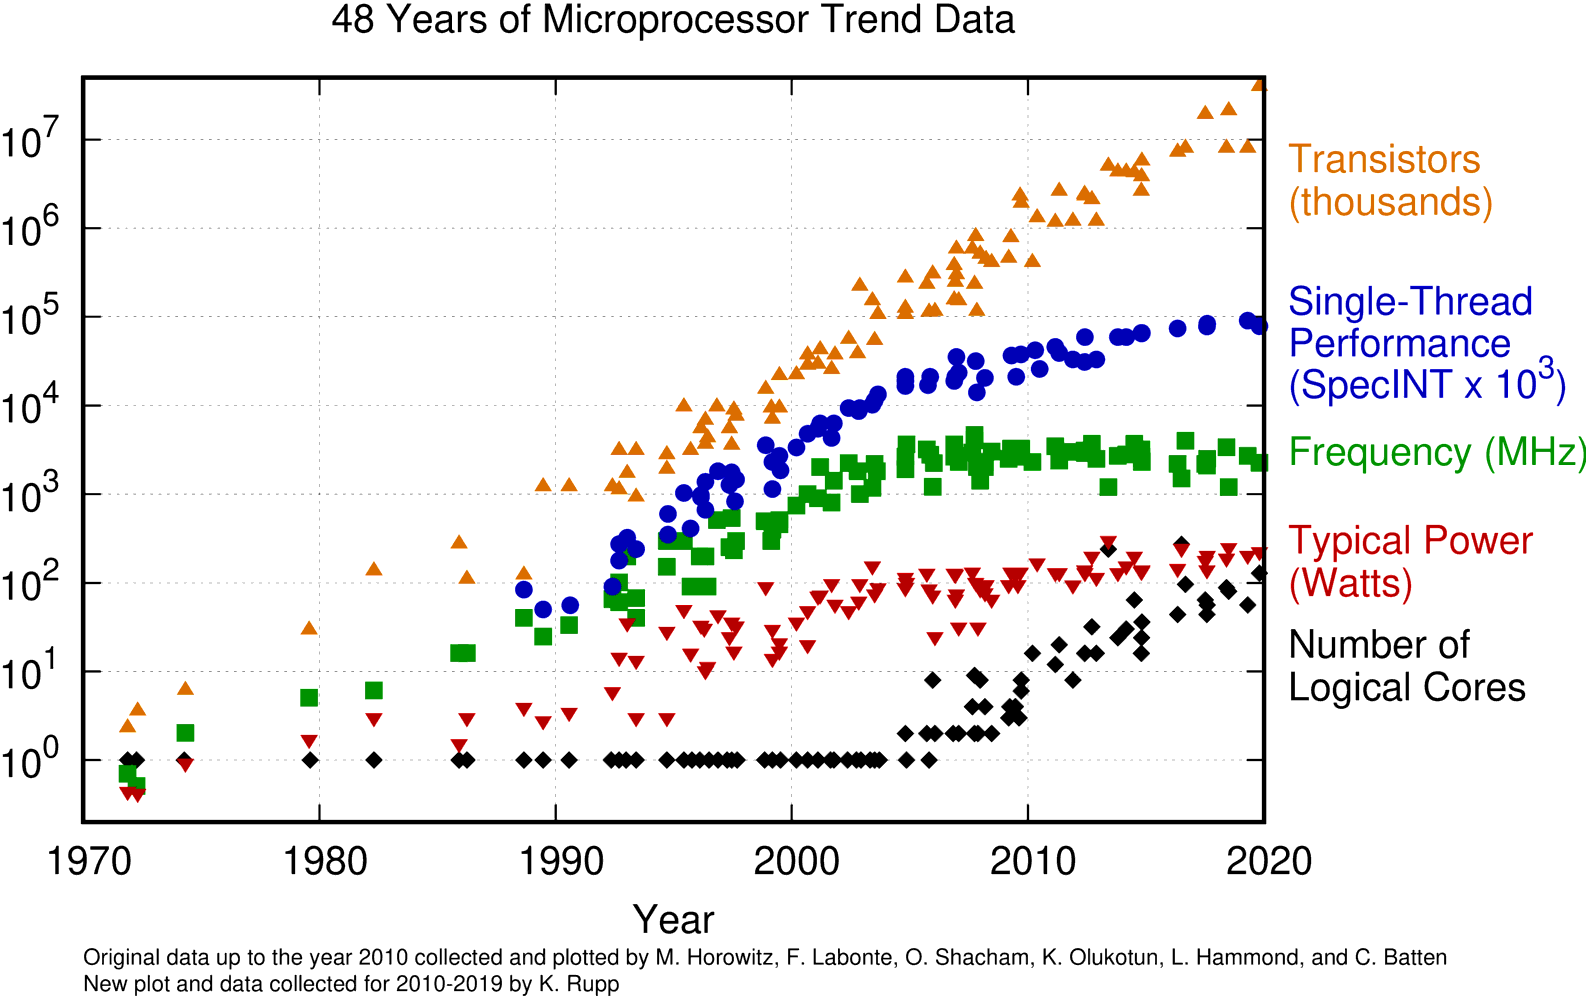
\includegraphics[height=.8\textheight]{images/48-years-processor-trend.png}}
      \mode<article>{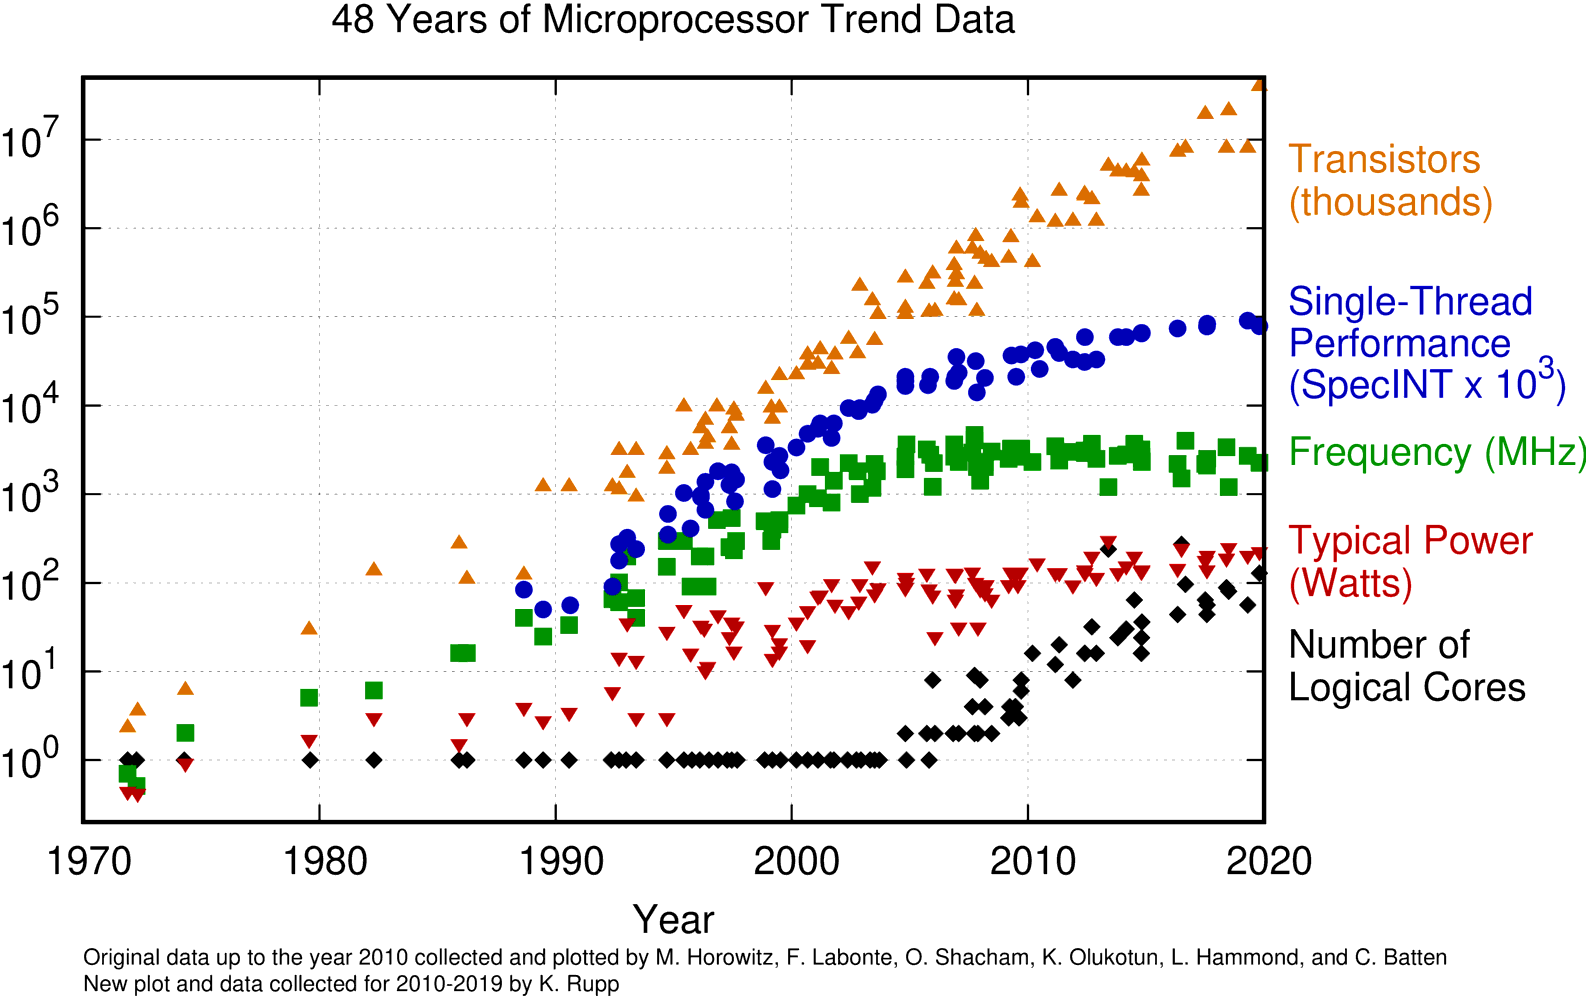
\includegraphics[height=.8\textwidth]{images/48-years-processor-trend.png}}
    \end{center}
\end{frame}

\begin{frame}[t]{The free lunch is over}
    \begin{itemize}
      \item Actividad: Lea completamente el artículo:
    \end{itemize}
    \vspace{2em}
    Fuente: \alert{The free lunch is over}.\\
    Herb Sutter.\\
    \url{http://www.gotw.ca/publications/concurrency-ddj.htm}\\
\end{frame}

\begin{frame}{Evolución del rendimiento}
\begin{columns}
  \begin{column}{.75\textwidth}
    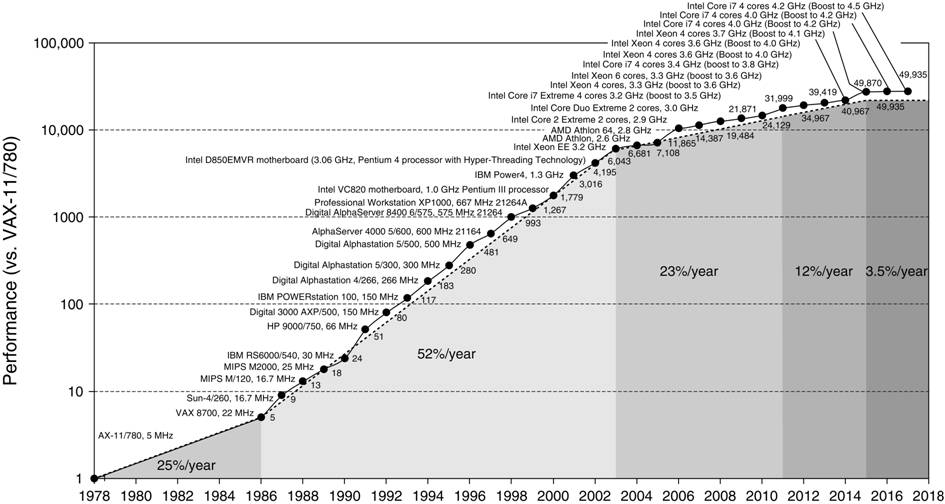
\includegraphics[width=\textwidth]{images/perf-evol.jpg}\\
    {\tiny Fuente: Computer Architecture: A Quantitative Approach. 5 Ed
Hennessy and Patterson. Morgan Kaufmann. 2012.}
  \end{column}
  \begin{column}[T]{.25\textwidth}
    \begin{itemize}
      \item 1986: \alert{RISC}.
      \item 2005: \alert{multi-core}.
    \end{itemize}
  \end{column}
\end{columns}
\end{frame}

\begin{frame}[t]{La revolución RISC}
\begin{itemize}
  \item Mejora continua de semiconductores ha dado lugar al dominio de computadores 
        basados en microprocesador.
    \mode<presentation>{\vfill}
    \begin{itemize}
      \item Desaparición de los minicomputadores.
      \mode<presentation>{\vfill}
      \item \emph{Mainframes} y supercomputadores construidos como colecciones de microprocesadores.
    \end{itemize}
  \mode<presentation>{\pause\vfill}
  \item Incremento sostenido del rendimiento de 1986 a 2003:
    \begin{itemize}
      \item \textbf{\alert{52\% anual}}.
    \end{itemize}
  \mode<presentation>{\pause\vfill}
  \item \textbf{¡Ha dejado de cumplirse!}
\end{itemize}
\end{frame}
